\documentclass[tikz,border=10pt]{standalone}
\begin{document}
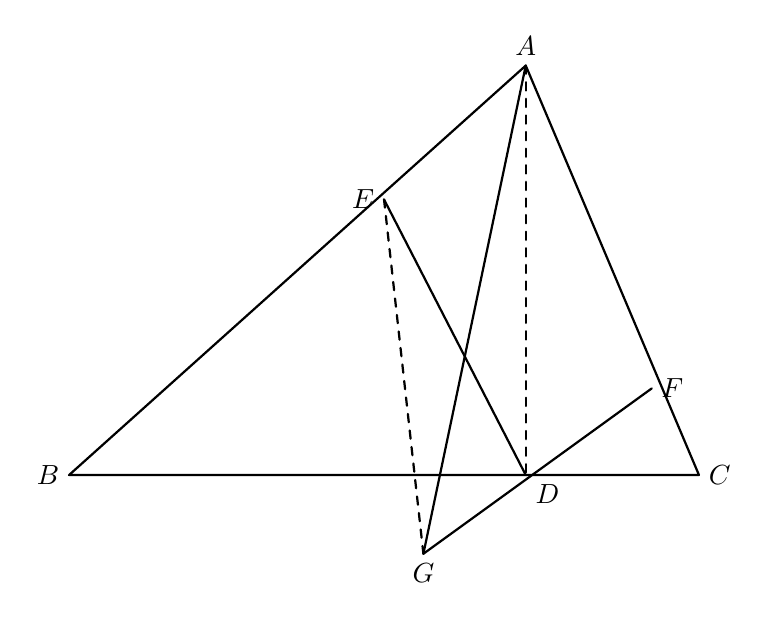
\begin{tikzpicture}[line cap=round,line join=round,scale=1]

\coordinate (B) at (0,0);
\coordinate (C) at (8,0);
\coordinate (A) at (5.8,5.2);
\coordinate (E) at (4.0,3.5);
\coordinate (D) at (5.8,0);
\coordinate (G) at (4.5,-1.0);
\coordinate (F) at (7.4,1.1);

\draw[thick] (B) -- (A) -- (C) -- (B);
\draw[thick] (E) -- (D);
\draw[thick] (A) -- (G);
\draw[thick] (G) -- (F);
\draw[dashed,thick] (E) -- (G);
\draw[dashed,thick] (A) -- (D);

\node[above] at (A) {$A$};
\node[left] at (B) {$B$};
\node[right] at (C) {$C$};
\node[below right] at (D) {$D$};
\node[left] at (E) {$E$};
\node[right] at (F) {$F$};
\node[below] at (G) {$G$};

\end{tikzpicture}
\end{document}
